\chapter{Introduction}
\section{Motivation}
Modern large scale spectroscopic surveys generate hundreds of thousands, or even millions of spectra. The analysis of these high volume data-sets presents a significant challenge to the researcher as well as to compute infrastructure and engineering. Additionally, if the data is collected by a high resolution instrument, the researcher will face the challenge of wrangling and analysing individual data points with dimensions at the scale of several thousands per spectrum \citep[e.g.,][]{buder2021galah+}. When the number of data points (i.e., spectra) is of the order of hundreds of thousands (or millions) and when each data point has a dimensionality of several thousands, it becomes impractical and perhaps even unfeasible to process and analyse these data using manual methods such as naked eye observations of spectral plots. 

In the case of stellar spectroscopic surveys, unless the science goals have been set to bias a survey specifically towards, for example, star forming regions  \citep{traven2015gaia}, these surveys will contain a majority of spectra that are presumably ``typical'', that is, with properties most common to the types of stars being targeted. Thus the identification and classification of {\em atypical} objects, such as emission-line stars, presents a serious challenge, in addition to those mentioned previously, as these spectra are outliers or anomalies in an otherwise typical set of stellar spectra.

\begin{table}[!htb]
\begin{center}
\begin{tabular}{|c|c|c|}
\hline
\textbf{Survey} & \textbf{Number of Spectra} & \textbf{Resolution} \\ \hline
Gaia ESO        & $\sim$150,000              & R$\sim$5000 to R$\sim$30,000             \\ \hline
LAMOST          & $\sim$10,000,000           & R$\sim$500 to R$\sim$1800              \\ \hline
APOGEE          & $\sim$250,000              & R$\sim$22,500             \\ \hline
RAVE            & $\sim$600,000              & R$\sim$7500                 \\ \hline
GAIA            & $\sim$100,000,000          & R$\sim$11,500 (RVS)               \\ \hline
\end{tabular}
\caption{Modern stellar spectroscopic surveys often generate large volumes of data, in some cases at high spectral resolution.}
\label{table:draglift1}
\end{center}
\end{table}
These surveys use data analysis pipelines to derive stellar parameters, and often use template spectra that represent typical or non-peculiar baselines. It has been demonstrated that the use of these so-called non-peculiar baselines can impact the accurate determination of effective temperature \citep{cayrel2011halpha, amarsi2018effective, giribaldi2019accurate} and stellar mass \citep{ness2016spectroscopic, bergemann2016gaia}, among other key measurements. The identification of atypical emission-line stars can thus help improve the accurate determination of these stellar parameters. To achieve this, once identified and classified, these spectra can be removed from the primary data analysis pipeline containing typical spectra, and can be reduced separately by secondary pipelines more suited for their peculiarities. 

The detection of atypical signals or data points in significantly larger, more typical populations of data presents itself well to modern machine-learning methods, particularly to anomaly detection, as well as to clustering methods (unsupervised learning). To date, a variety of machine-learning methods have been applied to the identification of emission-line stars, and in particular to H$\alpha$ emission-line stars. However, major drawbacks and challenges remain, for both the identification and the classification of emission-line stars, despite the use of popular and seemingly robust machine-learning methods such as dimensionality reduction, k-means clustering and neural networks. Given these challenges, it is not uncommon that manual methods are still being used for the identification and classification of emission-line stars even in modern data-sets with thousands of stars, with \citet{zhang2021catalog} being a recent example.  

In order to tackle the twin problems of identification and classification of emission-line stars, this work will apply unsupervised machine learning methods to data from the GALAH survey \citep{buder2021galah+}. The GALAH survey is a million-star high-resolution spectroscopic survey of the Milky Way which uses the HERMES spectrograph at the Anglo Australian Telescope \citep{de2015galah}. The most recent public data release from GALAH, Data Release 3 \citep[DR3;][]{buder2021galah+}), contains more than 600,000 high-resolution spectra. Motivated by the opportunities and challenges presented above, this work presents a novel data-driven approach to identify and classify emission-line stars in the GALAH database, utilising an unsupervised machine learning method that performs spectral-morphology-based clustering, with a particular focus on stars showing P Cygni and inverse P Cygni line H$\alpha$ profiles. However the methods presented in this work are sufficiently general that they can be applied to other atypical emission-line spectra, the details of which are provided in subsequent chapters. Additionally, considerable attention has been given to the use of computationally efficient algorithms, to ensure that the methods presented scale sufficiently beyond the size and scale of the GALAH survey and can be applied to other spectroscopic surveys where emission-line spectra are present. 

\section{A Note on P Cygni Line Profiles}

A principal line profile or feature that the reader will encounter in this work is the P Cygni line profile. P Cygni (or 34 Cygni) is a luminous blue variable star (LBV) that has been studied extensively \citep{1953PDAO....9....1B, hutchings1969expanding, elliott20225, underhill1966supergiants, mizumoto2018newly}. Willem Janszoon Blaeu, a Dutch cartographer and student of the astronomer Tycho Brahe, is considered to have provided the first known set of observations of 34 Cygni in the year 1600 \citep{de2001p}. The stellar spectrum of 34 Cygni is peculiar. It exhibits the characteristics of a B type supergiant except that almost all absorption lines are blueshifted with a redshifted emission component \citep{hutchings1969expanding}. This characteristic line profile can be clearly observed in proximity to the H$\alpha$ line whose rest wavelength is at $\sim 6562.7 {\rm \AA}$ \citep{zhang2021catalog, traven2015gaia}

P Cygni-type stars or more simply, P Cygni stars, are stars that exhibit line profiles that are similar to the characteristic profile of 34 Cygni. The spectra of these stars show characteristic absorption, emission and wide absorption sub-components \citep{zhang2021catalog}. The redshifted absorption (and blueshifted emission) counterparts to P Cygni stars have also been observed. These  belong to a class of objects known as inverse P Cygni stars. %or \emph{inverse P Cygni stars}. 

\begin{figure}[!htb]
\centering
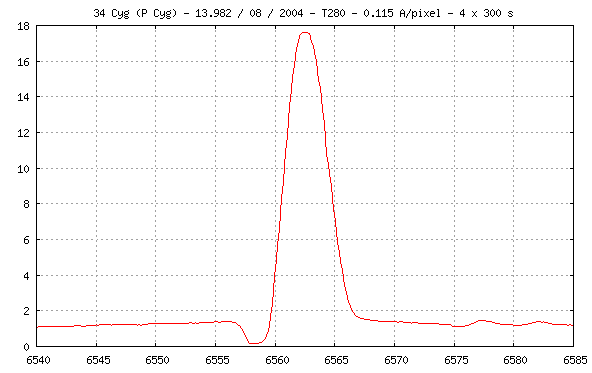
\includegraphics[scale=.60]{figures/34cygni.png}
\caption{The normalised spectrum of 34 Cygni around H$\alpha$.}
\end{figure}

It is believed that distinct physical processes within—and around—these stars generate the respective line profiles \citep{hou2016catalog}. Beals \citeyear{1953PDAO....9....1B} was the first to demonstrate that P Cygni and inverse P Cygni line profiles can be respectively explained by the interaction between the stellar disk of a hot, massive young star and the expanding—or contracting—shell of gas surrounding the star. 

\begin{figure}[!htb]
\centering
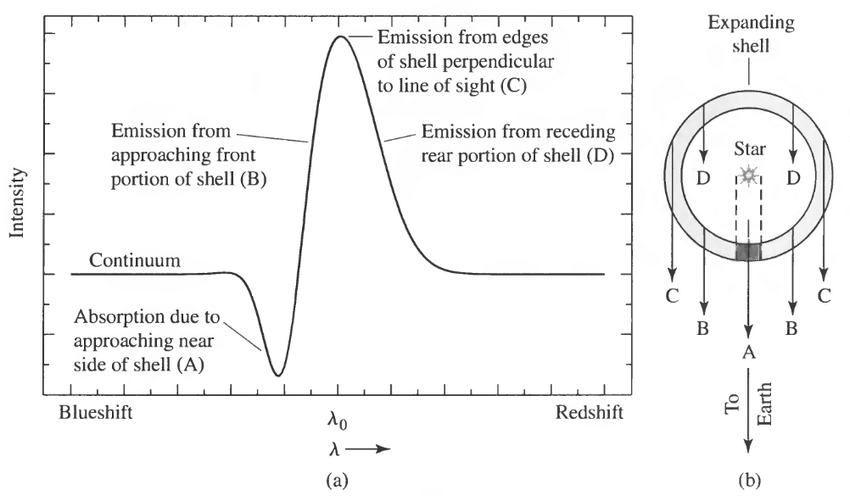
\includegraphics[scale=.52]{figures/expandingpcygni.png}
\caption{Cartoon depicting the physical mechanism by which a P Cygni line profile is generated. Reproduced from \citet{kasai2013type}.}
\label{fig1.2}
\end{figure}

An observed P Cygni line profile is thus a result of an expanding shell of gas around the main disk of the young hot star. The segment of this shell along the line of sight contributes to the generation of the absorption line in the spectrum. An average or "normal" main sequence star will only show a deep absorption line/trough near H$\alpha$. However, in the case of a P Cygni star, the regions B, C and D (in Figure \ref{fig1.2}) of the shell contribute to an emission line. This emission line can occur near H$\alpha$. As we move from B to C, the intensity of the emission line increases until we reach the edge of the shell. Beyond this point the shell is receding with respect to the line of sight and the intensity of the emission line consequently decreases. It is believed that the opposite process occurs in the case of an inverse P Cygni star. In this case, the shell of gas is contracting, and this inflow is responsible for the blueshifted emission line, often to the blueward of H$\alpha$. A full discussion of other classes of emission-line stars such as those presented in Figure \ref{fig1.3}, and the physics that generate the observed line profiles is beyond the scope of this thesis. However, this work will present suitable classes of such candidates in the GALAH survey where relevant, with the key motivation of this work being the identification of P Cygni and inverse P Cygni spectra in a survey that primarily contains typical spectra.

\begin{figure}[!htb]
\centering
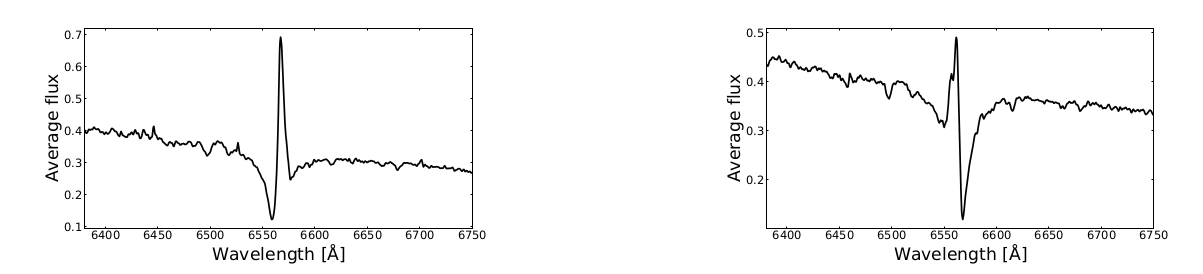
\includegraphics[scale=.50]{figures/p cygni and inverse p cygni.png}
\caption{Four general classes of emission-line spectra identified in the Gaia-ESO Survey. Reproduced from \citet{traven2015gaia}}
\label{fig1.3}
\end{figure}

\section{A Brief History of Classification}
One of the first modern attempts at the identification and classification emission-line stars, in particular P Cygni stars, was by \citet{1953PDAO....9....1B}. Beals compiled Northern Hemisphere observations of emission-line stars into a comprehensive catalogue. The catalogue was constructed by examining spectra visually, during a period of observation between the years 1928 and 1946. The data were then used to generate hypotheses of how P Cygni stars may exchange materials with their surroundings via accretion, inflows and outflows, and the morphological properties of the spectra were subsequently measured to calculate the wind velocities of inflows and outflows. Manual classification and visual observation of spectral plots was suitable in this context since the volume of data was not significant. However, such an approach would probably not be feasible in the modern era due to the reasons outlined above.

\begin{figure}[!htb]
\centering
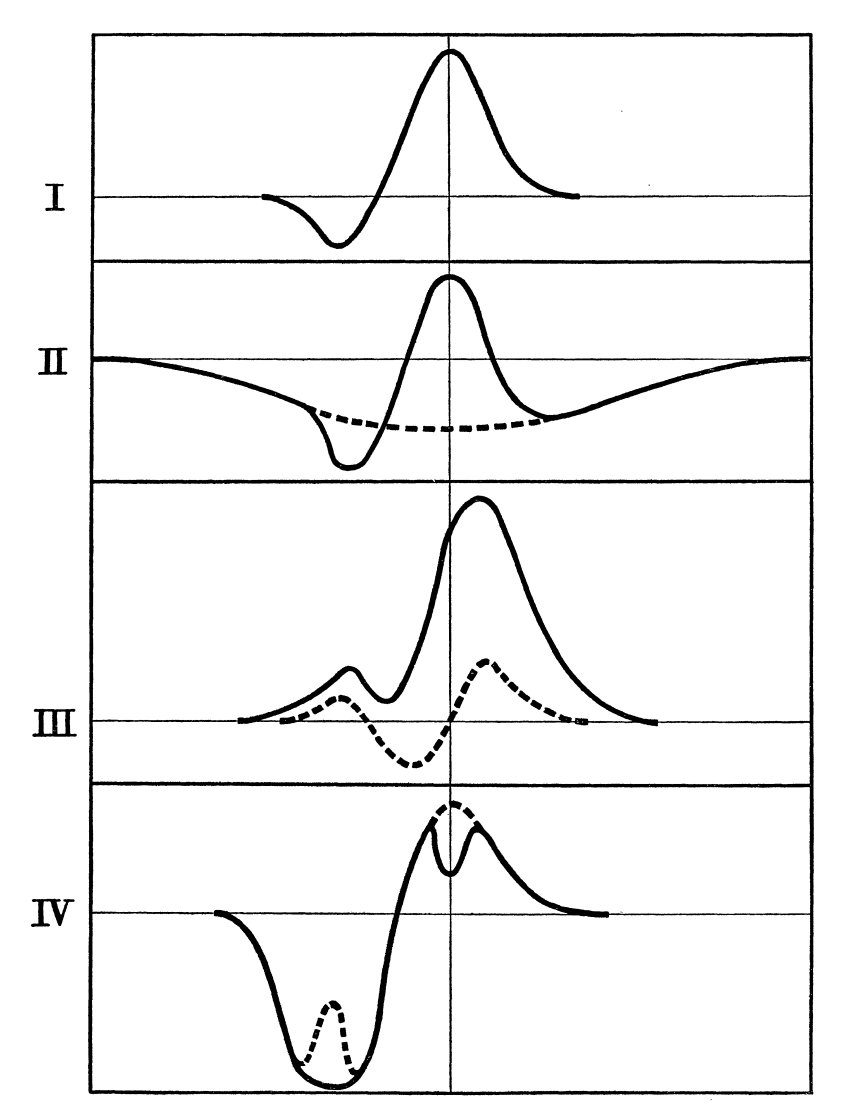
\includegraphics[scale=.35]{figures/beals class 1.png}
\caption{Primary classes of emission-line spectra proposed by \citet{1953PDAO....9....1B}.}
\end{figure}

Beals' work also presents an early attempt at classifying of emission-line stars based on their morphologies. The classification provided is simpler than more modern schemes, for example those presented in \citet{traven2015gaia}. In addition to what he labelled the primary classes, Beals proposed a set of non-typical classes, which were nonetheless also considered to be P Cygni spectra by Beals. In this work these non-typical classes are not treated as P Cygni spectra {\em per se}, but they are considered to be other classes of emission-line spectra. This approach is congruent with modern studies \citep[e.g.,][]{vcotar2021galah, zhang2021catalog, reipurth1996halpha} which place constraints on the classification of P Cygni and inverse P Cygni morphologies. 

It is worth noting that even subsequent work such as \citet{reipurth1996halpha} also relied on manual human classification of emission-line stars based on the morphological properties of the spectra. This remained a common practice towards the end of the 20th century, as the volume of data was not sufficiently large to warrant the use of data-driven and machine-learning-based classification routines. With the advent of large scale spectroscopic surveys, however, and significant advances in computational resources and machine learning methods, the stage was finally set for data-driven classification of machine-learning methods such as the use of t-SNE \citep{traven2017galah} and the application of neural networks as anomaly detectors \citep{vcotar2021galah}. But as this work will demonstrate, these methods are not sufficiently robust at identifying and classifying P Cygni, inverse P Cygni and other emission-line spectra. In order to overcome these challenges, this work will introduce a novel unsupervised machine-learning approach which will be discussed further in following chapters.

\begin{figure}[!htb]
\centering
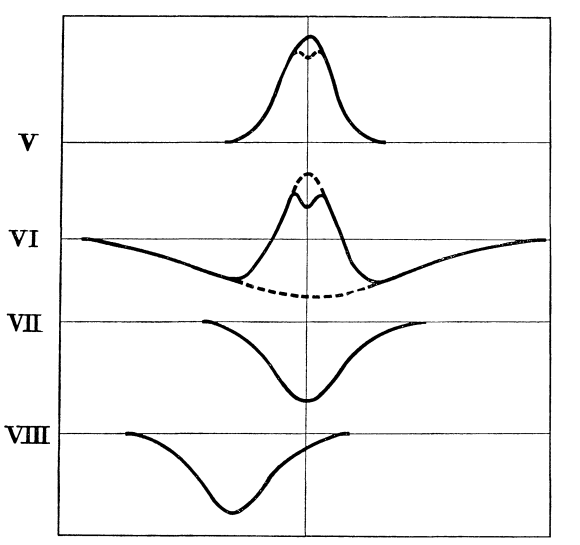
\includegraphics[scale=.50]{figures/beals class 2.png}
\caption{Secondary morphological classes proposed by Beals.}
\end{figure}

\section{Thesis Outline}

This thesis is structured as follows: Chapters 1 to 3 provide background on the problem statement, motivation, prior work and the data that were used in prototyping methods and deriving the results presented in the subsequent chapters. Chapters 4 to 6 provide detailed results as well as a comparison of this work to contemporary methods in the literature. The thesis concludes with Chapter 7, which places the results in context, provides a summarised commentary of the results and points out future directions of work. Conclusions have also been provided at the end of each chapter where relevant and appropriate. 

A detailed account of manual and machine learning-based methods to date is provided in Chapter 2, highlighting the relative advantages and disadvantages of these methods. Chapter 3 provides background regarding the DR3 data set, data preparation, re-sampling and feature engineering. In particular, Chapter 3 briefly introduces the concept of casting spectra as "time-series", which will be followed with a more detailed discussion in Chapter 4. Chapter 4 presents a novel data-driven approach that exploits this concept to identify, cluster and classify emission-line spectra. This chapter will demonstrate the efficacy of this approach on a sample of data from a recent study by \citet{vcotar2021galah}. 

Chapter 5 compares the approach developed in Chapter 4 with a recent and popular machine-learning method known as t-SNE. t-SNE was introduced as a suitable method to classify a broad range of spectral types in the GALAH survey. One of the conclusions of this chapter is that t-SNE is not sufficiently effective at identifying and classifying emission-line spectra. In particular, this work will demonstrate that the novel approach presented in Chapter 4 is more effective than t-SNE for the classification of P Cygni, inverse P Cygni and other emission-line spectra.

Chapter 6 builds on insights from chapters 3, 4 and 5 and introduce an end-to-end data driven machine learning method which ingests GALAH survey data, extracts emission-line spectra and classifies P Cygni, inverse P Cygni and other emission-line spectra. Using this novel approach, this work found over 7,000 emission-line spectra, over 200 P Cygni spectra and 200 inverse P Cygni spectra. The key results and ideas for building upon this work in the future are presented in Chapter 7.

